\documentclass{article}
\usepackage{tikz}

\begin{document}

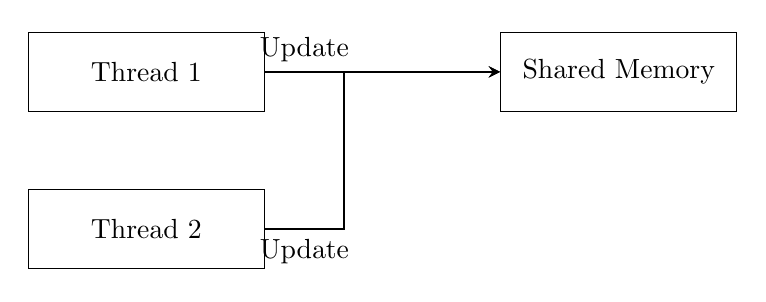
\begin{tikzpicture}[node distance=2cm]

    % Define styles for nodes and arrows
    \tikzset{
        box/.style={rectangle, draw=black, fill=white, text centered, minimum width=3cm, minimum height=1cm},
        line/.style={->, thick, >=stealth}
    }

    % Nodes representing the threads of execution
    \node (thread1) [box] {Thread 1};
    \node (thread2) [box, below of=thread1] {Thread 2};

    % Nodes representing the shared memory
    \node (sharedMemory) [box, right of=thread1, xshift=4cm] {Shared Memory};

    % Arrows connecting the threads to the shared memory
    \draw [line] (thread1.east) -- node[above] {Update} ++(1,0) |- (sharedMemory.west);
    \draw [line] (thread2.east) -- node[below] {Update} ++(1,0) |- (sharedMemory.west);

\end{tikzpicture}

\end{document}